\documentclass[border=15pt, multi, tikz]{article}
\usepackage[backend=bibtex,style=authoryear,natbib=true]{biblatex} % Use the bibtex backend with the authoryear citation style (which resembles APA)

\addbibresource{example.bib} % The filename of the bibliography

\usepackage[autostyle=true]{csquotes} % Required to generate language-dependent quotes in the bibliography
\usepackage{import}
\usepackage{tikz}
\usepackage{tikz-network}
\usetikzlibrary{calc,patterns,angles,quotes}
\usepackage{breqn}
\usepackage{bm}
\usepackage{float}
\usepackage{graphicx}
\usepackage{subcaption}
\usepackage{multirow}
\usepackage{graphicx}
\usepackage{rotating}
\usetikzlibrary{fit}
\usetikzlibrary {arrows.meta,graphs,shapes.misc}
\usetikzlibrary {positioning}
\subimport{./layers/}{init}
\newcommand{\bn}{\textbf{n}}
\newcommand{\tabhead}[1]{\textbf{#1}}

\def\ConvColor{rgb:yellow,5;red,2.5;white,5}
\def\ConvReluColor{rgb:yellow,5;red,5;white,5}
\def\PoolColor{rgb:red,1;black,0.3}
\def\DcnvColor{rgb:blue,5;green,2.5;white,5}
\def\SoftmaxColor{rgb:magenta,5;black,7}
\def\SumColor{rgb:blue,5;green,15}
\def\poolsep{1}


\begin{document}

\section{Training Details}

The approaches are trained on dataset "synthetic-50-5" as mentioned in Chapter \ref{ch:04} with 3000 scenes. Each scene has a depth map with dimension $ 128\times 128 \times $ in height, width and channel, an image with dimension $ 128\times 128 \times 1 $.  The depth map is converted to 3D vertex map as introduced in Chapter \ref{ch:04}. The light map is calculated based on vertex map and the known light position. We create a tensor in PyTorch that includes vertex map, image and the light direction for each scene and considered it as one training case. Thus 3000 scenes has corresponding 3000 training cases. Each scene has a corresponding ground-truth normal map for loss calculation and the evaluation. 

The training processes are evaluated in every 100 epochs with 29 evaluation scenes that model never seen before, which contains the 5 different objects in the ``synthetic-50-5" test set. Figure \ref{fig:test-scene} shows some of the test scenes during the training work.

\begin{figure}[H]
	\centering
	
		\begin{subfigure}[b]{0.18\linewidth}
		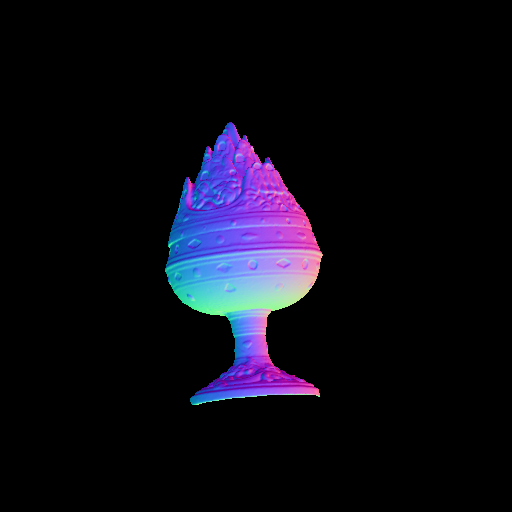
\includegraphics[width=\linewidth]{./Figures/test_scenes/05051.normal0.png}
	\end{subfigure}
	\begin{subfigure}[b]{0.18\linewidth}
		\includegraphics[width=\linewidth]{./Figures/test_scenes/05109.normal0.png}
	\end{subfigure}
	\begin{subfigure}[b]{0.18\linewidth}
		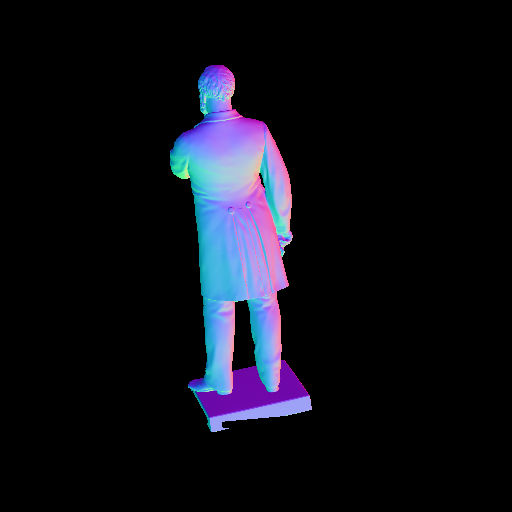
\includegraphics[width=\linewidth]{./Figures/test_scenes/05111.normal0.png}
	\end{subfigure}
	\begin{subfigure}[b]{0.18\linewidth}
		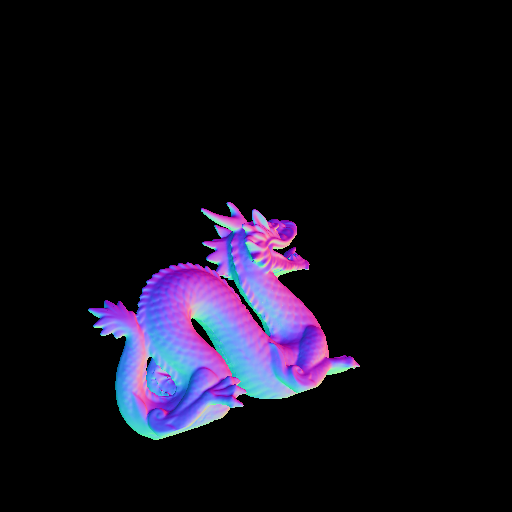
\includegraphics[width=\linewidth]{./Figures/test_scenes/05113.normal0.png}
	\end{subfigure}
	\begin{subfigure}[b]{0.18\linewidth}
		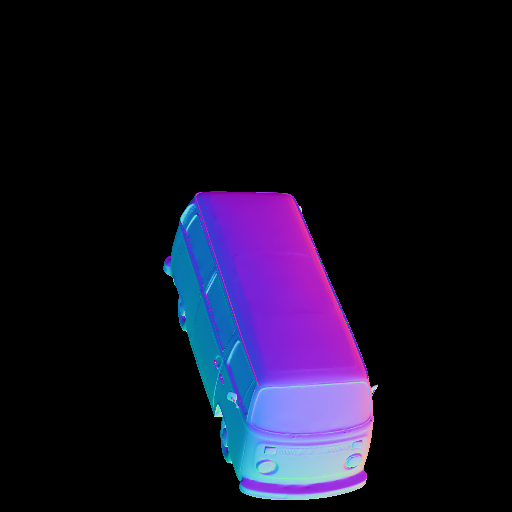
\includegraphics[width=\linewidth]{./Figures/test_scenes/05126.normal0.png}
	\end{subfigure}
	
	
	\begin{subfigure}[b]{0.18\linewidth}
		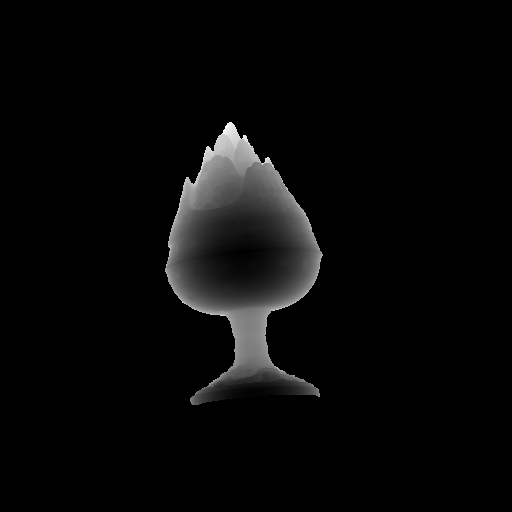
\includegraphics[width=\linewidth]{./Figures/test_scenes/05051.depth0.png}
	\end{subfigure}
	\begin{subfigure}[b]{0.18\linewidth}
		\includegraphics[width=\linewidth]{./Figures/test_scenes/05109.depth0.png}
	\end{subfigure}
	\begin{subfigure}[b]{0.18\linewidth}
		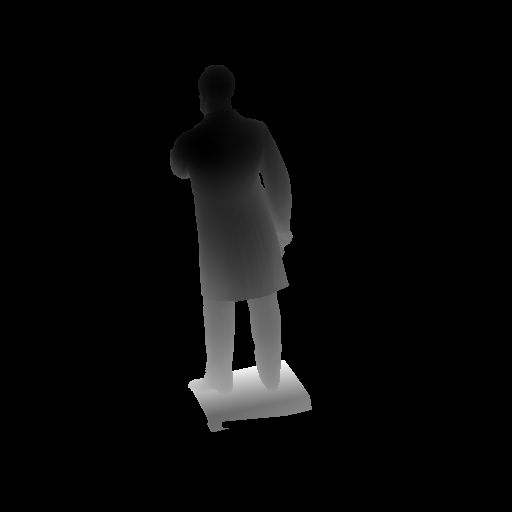
\includegraphics[width=\linewidth]{./Figures/test_scenes/05111.depth0.png}
	\end{subfigure}
	\begin{subfigure}[b]{0.18\linewidth}
		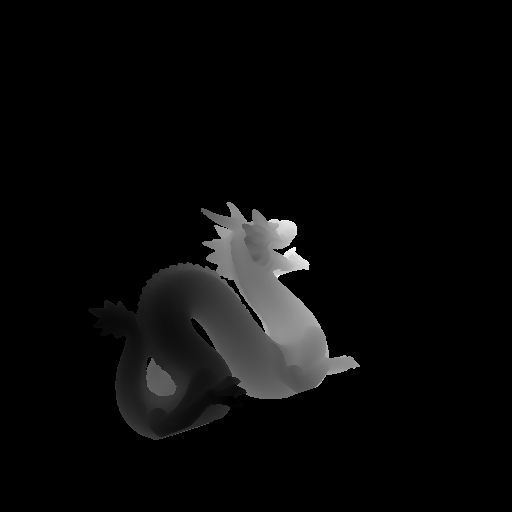
\includegraphics[width=\linewidth]{./Figures/test_scenes/05113.depth0.png}
	\end{subfigure}
	\begin{subfigure}[b]{0.18\linewidth}
		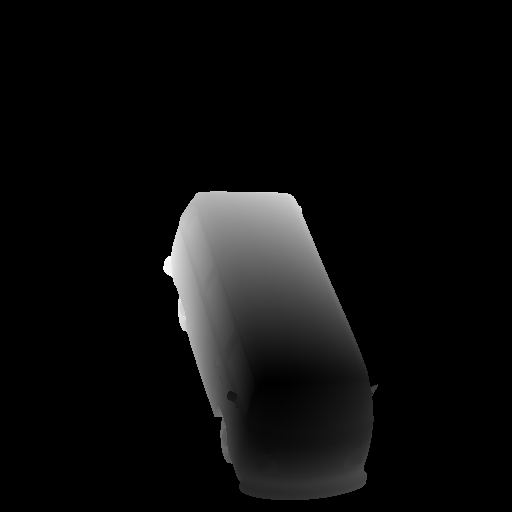
\includegraphics[width=\linewidth]{./Figures/test_scenes/05126.depth0.png}
	\end{subfigure}

	\begin{subfigure}[b]{0.18\linewidth}
	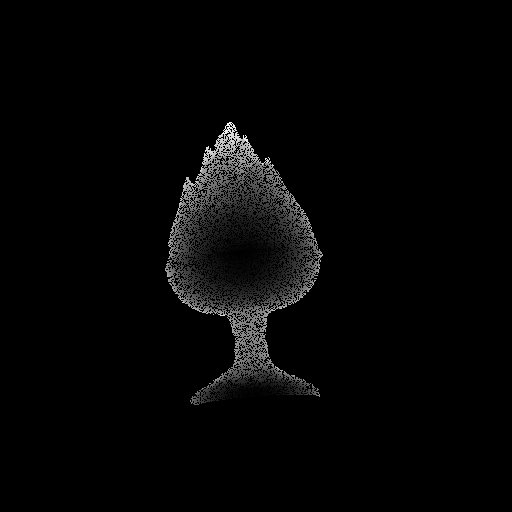
\includegraphics[width=\linewidth]{./Figures/test_scenes/05051.depth0_noise.png}
\end{subfigure}
\begin{subfigure}[b]{0.18\linewidth}
	\includegraphics[width=\linewidth]{./Figures/test_scenes/05109.depth0_noise.png}
\end{subfigure}
\begin{subfigure}[b]{0.18\linewidth}
	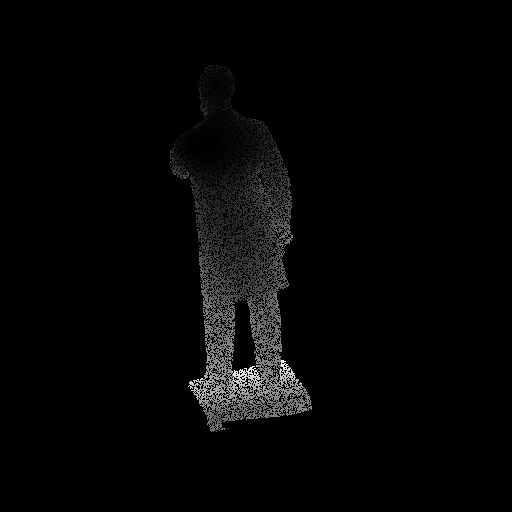
\includegraphics[width=\linewidth]{./Figures/test_scenes/05111.depth0_noise.png}
\end{subfigure}
\begin{subfigure}[b]{0.18\linewidth}
	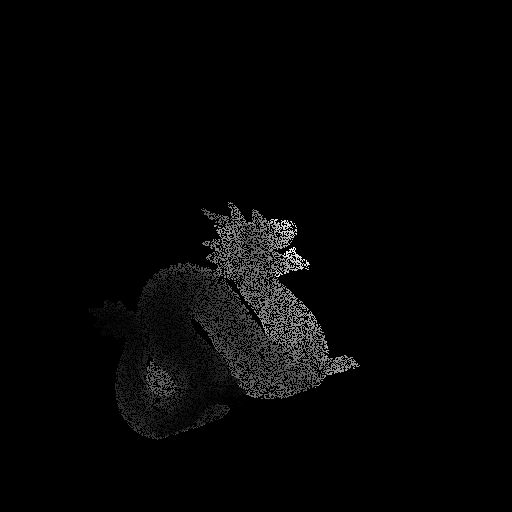
\includegraphics[width=\linewidth]{./Figures/test_scenes/05113.depth0_noise.png}
\end{subfigure}
\begin{subfigure}[b]{0.18\linewidth}
	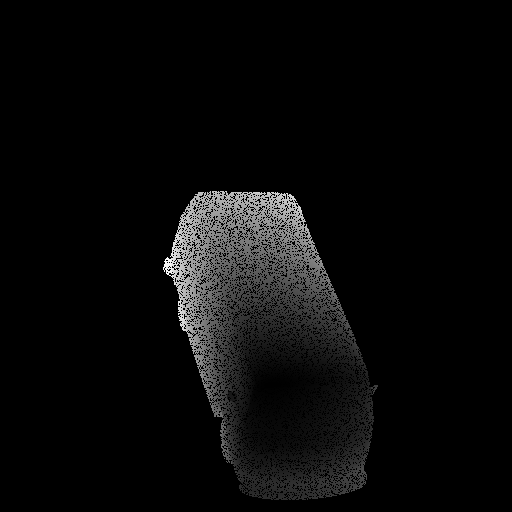
\includegraphics[width=\linewidth]{./Figures/test_scenes/05126.depth0_noise.png}
\end{subfigure}

	
	\begin{subfigure}[b]{0.18\linewidth}
		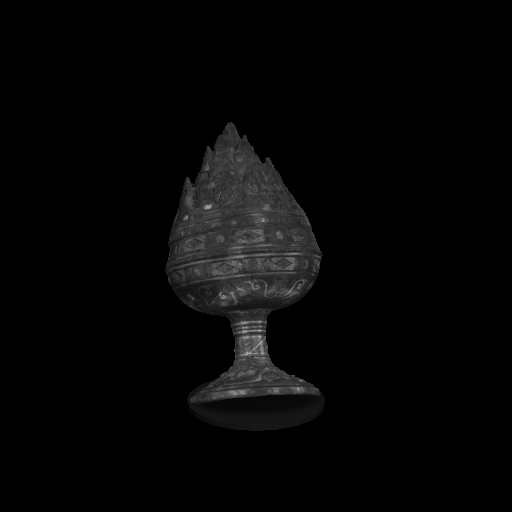
\includegraphics[width=\linewidth]{./Figures/test_scenes/05051.image0.png}
		\caption{Baoshanlu}
	\end{subfigure}
	\begin{subfigure}[b]{0.18\linewidth}
		\includegraphics[width=\linewidth]{./Figures/test_scenes/05109.image0.png}
		\caption{Vase}
	\end{subfigure}
	\begin{subfigure}[b]{0.18\linewidth}
		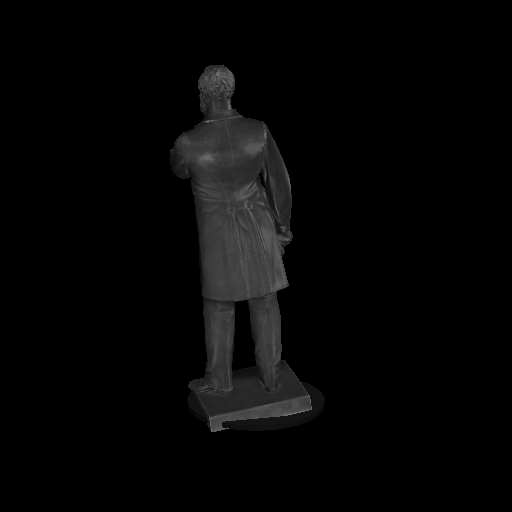
\includegraphics[width=\linewidth]{./Figures/test_scenes/05111.image0.png}
		\caption{Garfield}
	\end{subfigure}
	\begin{subfigure}[b]{0.18\linewidth}
		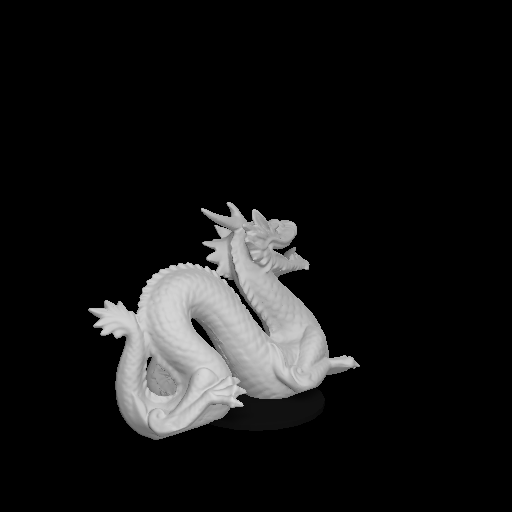
\includegraphics[width=\linewidth]{./Figures/test_scenes/05113.image0.png}
		\caption{Dragon}
	\end{subfigure}
	\begin{subfigure}[b]{0.18\linewidth}
		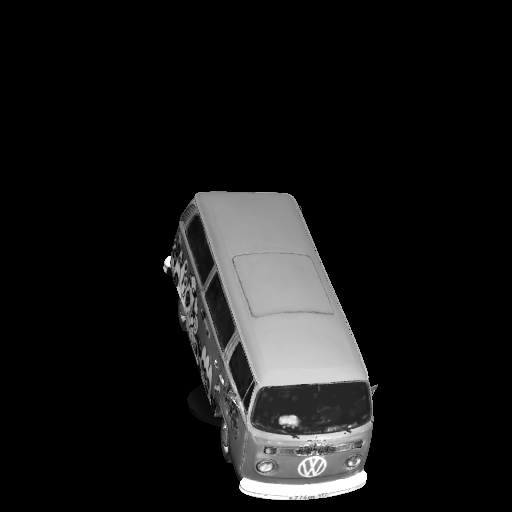
\includegraphics[width=\linewidth]{./Figures/test_scenes/05126.image0.png}
		\caption{Bus}
	\end{subfigure}	
	\caption{Some of the test scenes during the training. From top to bottom, normal map, depth map, noised depth map, grayscale image.}
	\label{fig:test-scene}
\end{figure}

The training pipeline use batch size $ 8 $,  Adam optimizer (\cite{adam}), learning rate start from  $ 1\times10^{-3} $, learning schedule [8,1000], learning decay factor 0.5. The model is trained with PyTorch 1.10.0a0, CUDA 11.4.1, GPU with single NVIDIA GEFORCE RTX 3090. It takes 14 hours to train GCNN and 35 hours to train the Trip-Net. We terminate the training when the evaluation on the test dataset converged.


\section{GCNN model evaluation based on Geometry Information}
The GCNN model is the base model of the whole thesis. The architecture is described in \ref{sec:gcnn}. We use a single GCNN to estimate the surface normal based on geometry information. It uses vertex map as input to estimate the corresponding tangent surface normal map. 

In order to verify the applicability of UNet architecture and Gated Convolution layer for the normal inference task, two similar models are created. 
We replace all of the gated layer to standard convolution layers in the network but keeps all of the other settings same in model ``CNN". It is used to verify the performance the gated convolution layers. As mentioned in chapter \ref{ch:03}, the gated layer is designed to deal with noised input. Since all of the vertex map in the dataset has been added noise, the GCNN is supposed to over-perform ``CNN". Another model called ``NOC" is designed to verify the skip connection in the UNet, which simply removes the skip connections in the network but keeps other settings same. Is is designed to show the validation of skip connections. Figure \ref{fig:gcnn-training-history} shows the training history on BerHu Loss. The GCNN approach achieves a lower loss from start to the end of the training.

\begin{figure}[th]
	\centering
	\includegraphics[width=.8\textwidth]{./Figures/gcnn_loss_compare.png}
	\caption{The training history of GCNN model. The line chart records the training BerHu loss of the model GCNN, NOC and CNN.}
	\label{fig:gcnn-training-history}
\end{figure}




%% gcnn-eval
\begin{figure}[H]
	\centering
	\begin{subfigure}[b]{0.18\linewidth}
		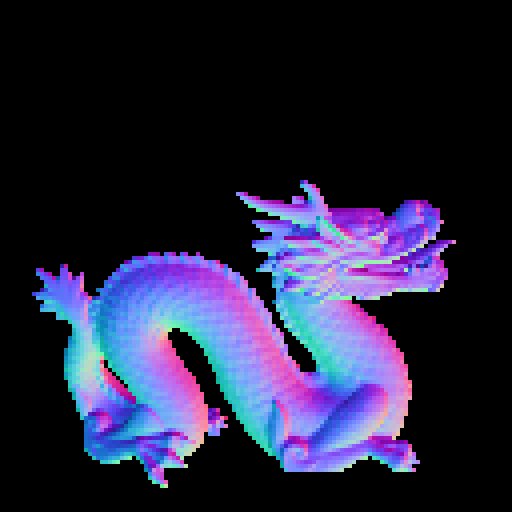
\includegraphics[width=\linewidth]{./Figures/visual_eval/fancy_eval_7_groundtruth.png}
	\end{subfigure}
	\begin{subfigure}[b]{0.18\linewidth}
		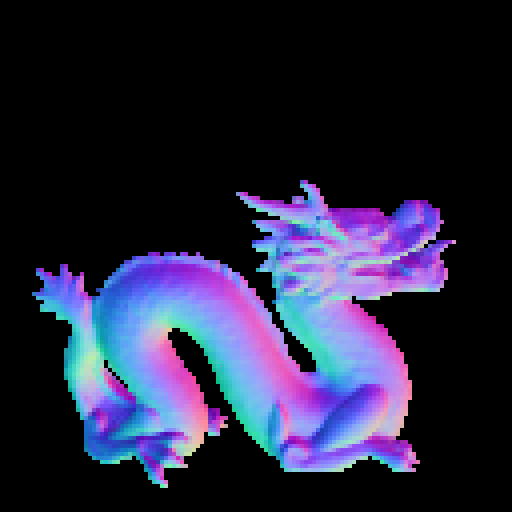
\includegraphics[width=\linewidth]{./Figures/visual_eval/fancy_eval_7_normal_GCNN-GCNN.png}
	\end{subfigure}
	\begin{subfigure}[b]{0.18\linewidth}
		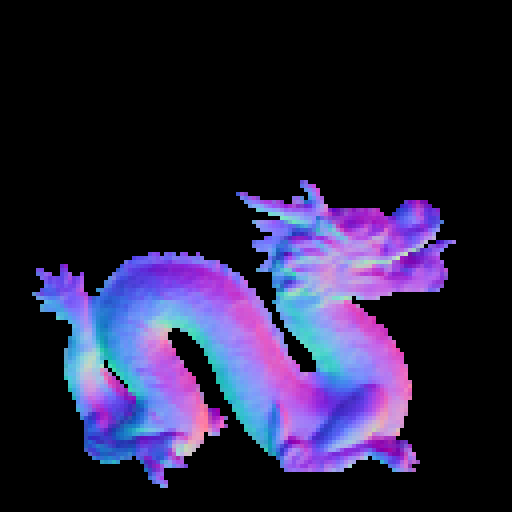
\includegraphics[width=\linewidth]{./Figures/visual_eval/fancy_eval_7_normal_GCNN-CNN.png}
	\end{subfigure}
	\begin{subfigure}[b]{0.18\linewidth}
		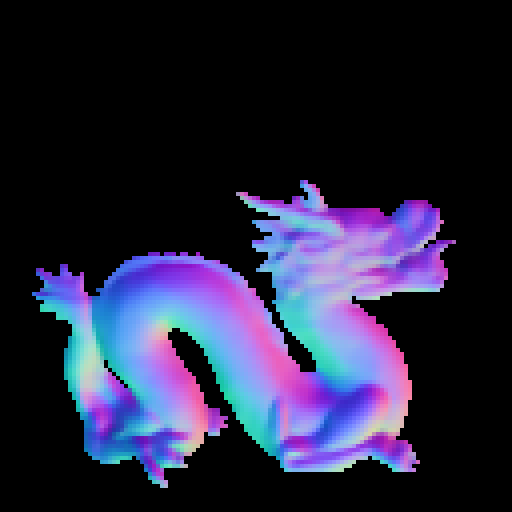
\includegraphics[width=\linewidth]{./Figures/visual_eval/fancy_eval_7_normal_GCNN-NOC.png}
	\end{subfigure}
	\begin{subfigure}[b]{0.18\linewidth}
		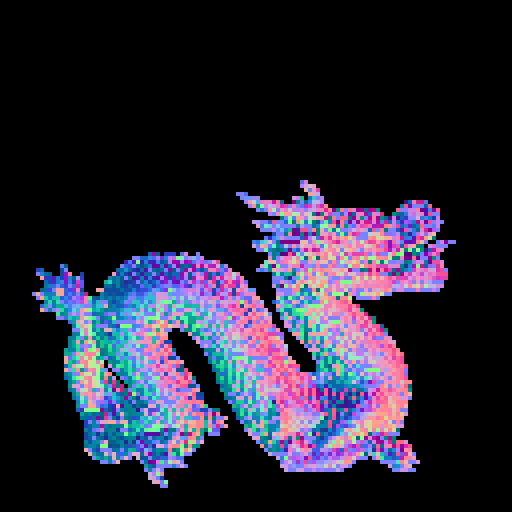
\includegraphics[width=\linewidth]{./Figures/visual_eval/fancy_eval_7_normal_SVD.png}
	\end{subfigure}
	
	\begin{subfigure}[b]{0.18\linewidth}
		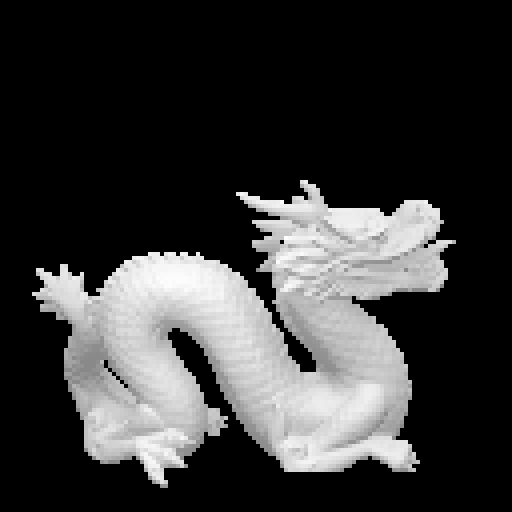
\includegraphics[width=\linewidth]{./Figures/visual_eval/fancy_eval_7_img.png}
		\caption{GT}
	\end{subfigure}
	\begin{subfigure}[b]{0.18\linewidth}
		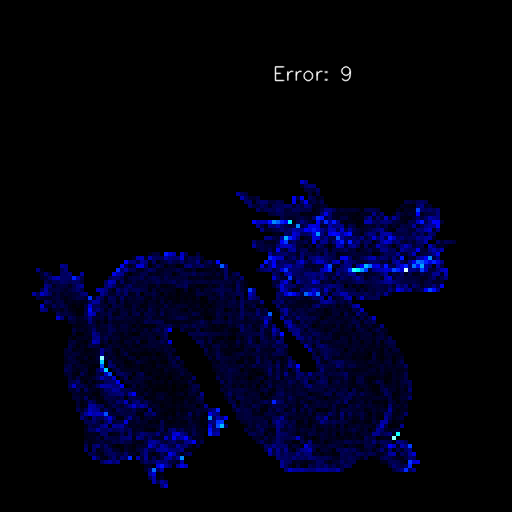
\includegraphics[width=\linewidth]{./Figures/visual_eval/fancy_eval_7_error_GCNN-GCNN.png}
		\caption{GCNN}
	\end{subfigure}
	\begin{subfigure}[b]{0.18\linewidth}
		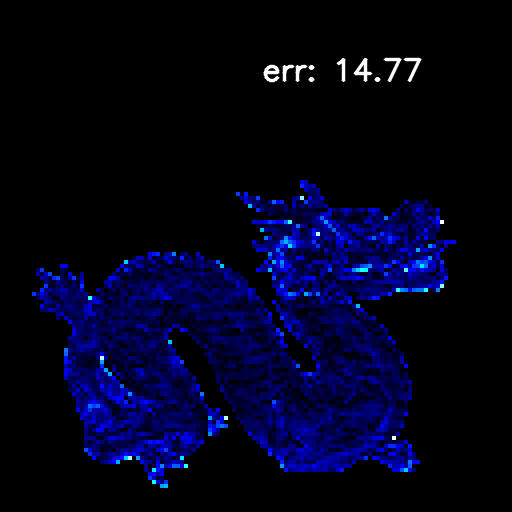
\includegraphics[width=\linewidth]{./Figures/visual_eval/fancy_eval_7_error_GCNN-CNN.png}
		\caption{CNN}
	\end{subfigure}
	\begin{subfigure}[b]{0.18\linewidth}
		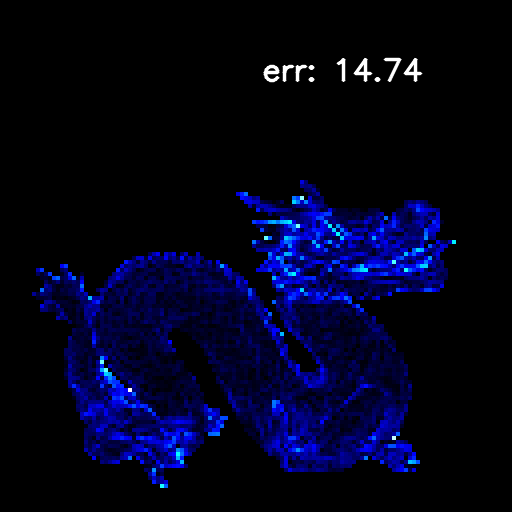
\includegraphics[width=\linewidth]{./Figures/visual_eval/fancy_eval_7_error_GCNN-NOC.png}
		\caption{NOC}
	\end{subfigure}
	\begin{subfigure}[b]{0.18\linewidth}
		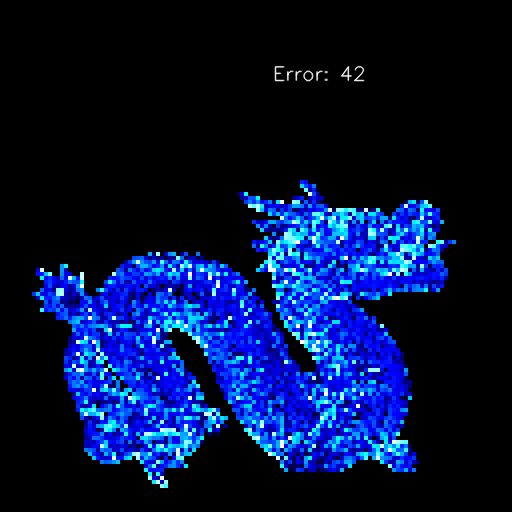
\includegraphics[width=\linewidth]{./Figures/visual_eval/fancy_eval_7_error_SVD.png}
		\caption{SVD}
	\end{subfigure}
	
	\begin{tikzpicture}
		\node[text width=0.1\textwidth] at (10,-1) {90};
		\node[inner sep=0pt] (input) at (8,-1)
		{
\includegraphics[width=.2\textwidth]{./Figures/colorscale_blue.png}};
		\node[text width=0.3\textwidth] at (7,-1) {Error: 0};
	\end{tikzpicture}
	
	\caption{Surface Normal Inference based GCNN model on "Dragon´´ object. The first row shows the estimated surface normal. The second row is the angle error map.}
	\label{fig:gcnn-eval}
\end{figure}


A qualitative evaluation on object "dragon" is shown in Figure \ref{fig:gcnn-eval}. SVD approach is considered as the baseline shown in last column. As shown in the figure, learning based methods performs better than SVD in terms of angle error. The SVD approach is failed to deal with semi-dense input since there exists many points that missing neighbors. The GCNN model is especially good at noise input due to the gated convolution layer design. As a further detailed comparison, \ref{fig:gcnn-eval-synthetic-zoom-in} gives a closer visualization on the same object. 



%% fig:gcnn-eval-synthetic-zoom-in
\begin{figure}[H]
	\centering
	\begin{subfigure}[b]{0.18\linewidth}
		\includegraphics[width=\linewidth]{./Figures/visual_eval/eval_7_normal_GT.png}
	\end{subfigure}
	\begin{subfigure}[b]{0.18\linewidth}
		\includegraphics[width=\linewidth]{./Figures/visual_eval/eval_7_normal_GCNN-GCNN.png}
	\end{subfigure}
	\begin{subfigure}[b]{0.18\linewidth}
		\includegraphics[width=\linewidth]{./Figures/visual_eval/eval_7_normal_GCNN-NOC.png}
	\end{subfigure}
	\begin{subfigure}[b]{0.18\linewidth}
		\includegraphics[width=\linewidth]{./Figures/visual_eval/eval_7_normal_GCNN-CNN.png}
	\end{subfigure}
	\begin{subfigure}[b]{0.18\linewidth}
		\includegraphics[width=\linewidth]{./Figures/visual_eval/eval_7_normal_SVD.png}
	\end{subfigure}
	
	\begin{subfigure}[b]{0.18\linewidth}
		\includegraphics[width=\linewidth]{./Figures/visual_eval/eval_7_img.png}
		\caption{GT}
	\end{subfigure}
	\begin{subfigure}[b]{0.18\linewidth}
		\includegraphics[width=\linewidth]{./Figures/visual_eval/eval_7_error_GCNN-GCNN.png}
		\caption{GCNN}
	\end{subfigure}
	\begin{subfigure}[b]{0.18\linewidth}
		\includegraphics[width=\linewidth]{./Figures/visual_eval/eval_7_error_GCNN-NOC.png}
		\caption{NOC}
	\end{subfigure}
	\begin{subfigure}[b]{0.18\linewidth}
		\includegraphics[width=\linewidth]{./Figures/visual_eval/eval_7_error_GCNN-CNN.png}
		\caption{CNN}
	\end{subfigure}
	\begin{subfigure}[b]{0.18\linewidth}
		\includegraphics[width=\linewidth]{./Figures/visual_eval/eval_7_error_SVD.png}
		\caption{SVD}
	\end{subfigure}
	
	\caption{Zoom in of the center region of Dragon object. The first row is surface normal, the second row is the corresponding errors. NOC model has no skip connnection, CNN model replace gated convolution layer to standard convolution layer.}
	\label{fig:gcnn-eval-synthetic-zoom-in}
\end{figure}
As shown in figure \ref{fig:gcnn-eval-synthetic-zoom-in}, the GCNN method gives a sharper edge prediction on the horn area of the dragon object, as well as the scales, whereas the no skip version (NOC) is blurry in the same area.

The CNN version has the skip connection thus gives a better detail than NOC model. However, if we compare the error map of GCNN and CNN in figure \ref{fig:gcnn-eval}, the CNN has less accurate in the smooth area than GCNN model. Like the dragon body, CNN model has a overall higher error than GCNN. It is because the noise of the input still disturb the CNN model and it takes the input noise into account for normal estimation which deviate to the correct surface normal. When we look back to the GCNN based method, we can found that the surface normal has better performance in the smooth area compare to the CNN approach and a sharp detail compare to the no skip connection version.

Table \ref{tab:gcnn-eval} gives a quantitative evaluation for GCNN model. It bases on 100 different test scenes in the "synthetic-50-5´´ dataset with angle metrics for evaluation.



\begin{table}[H]
	
	\centering
	\begin{tabular}{l l l l l l }
		\tabhead{Model} & \tabhead{Angle} & \tabhead{Time /ms} & \tabhead{bz} & \tabhead{lr-schedule} & \tabhead{lr-df}\\
		SVD(baseline)  & 41.14  & 320.40 & 8 & 8,1000 & 0.5\\ 
		\hline
		GCNN  & 10.64  & 10.44 & 8 & 8,1000 & 0.5\\ 
		\hline
		GCNN-NOC & 13.61 & 5.38 & 8 & 8,1000 & 0.5\\
		\hline
		CNN & 15.35 & 4.15 & 8 & 8,1000 & 0.5\\
	\end{tabular}
	\caption{The performance of the GCNN model for geometry information based normal inference. The angle error is the average angle error of all valid pixels in the test case. bz stands for batch size, lr-schedule stands for learning rate schedule, lr-df stands for learning rate decay factor.}	
	\label{tab:gcnn-eval}
\end{table}





\newpage
\section{Surface Normal Inference based on Calibrated Illuminated RGBD images }

For the approach using illuminated calibrated RGBD image, the task is undertaken by Trip-Net introduced in \ref{sec:trip-net}. 
The qualitative evaluation is shown in figure \ref{fig:trip-eval}. As a comparison, we placed GCNN result in the last column. The training settings for all the models are exact the same to ensure fairness. As shown in the figure, TripNet uses illuminated calibrated RGBD image has a better performance than GCNN model. The dragon scales are sharper in TripNet result. Figure \ref{fig:tripnet-eval-synthetic-zoom-in} gives a closer visualization.
%% TripNet-eval
\begin{figure}[H]
	\centering
	\begin{subfigure}[b]{0.18\linewidth}
		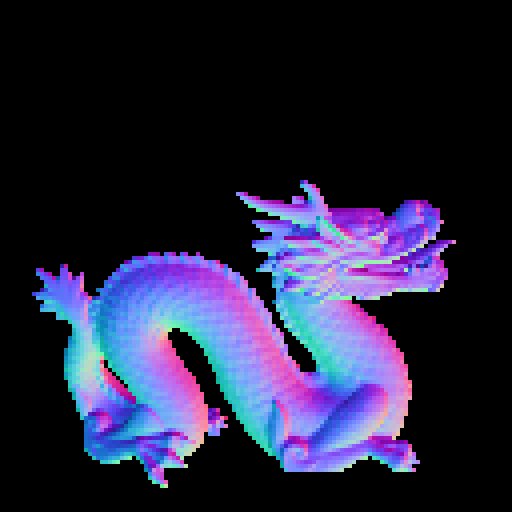
\includegraphics[width=\linewidth]{./Figures/visual_eval/fancy_eval_7_groundtruth.png}
	\end{subfigure}
	\begin{subfigure}[b]{0.18\linewidth}
		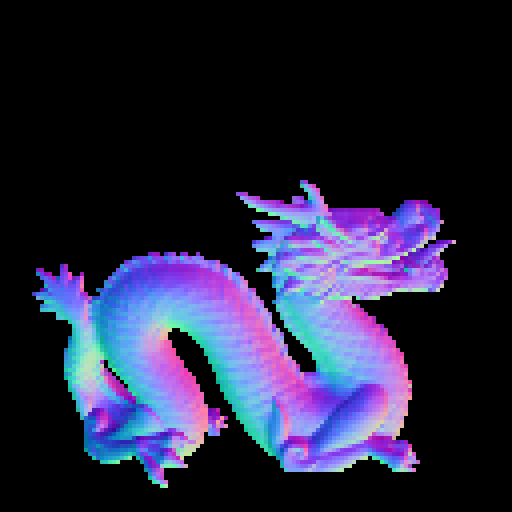
\includegraphics[width=\linewidth]{./Figures/visual_eval/fancy_eval_7_normal_an2-8-1000.png}
	\end{subfigure}
	\begin{subfigure}[b]{0.18\linewidth}
	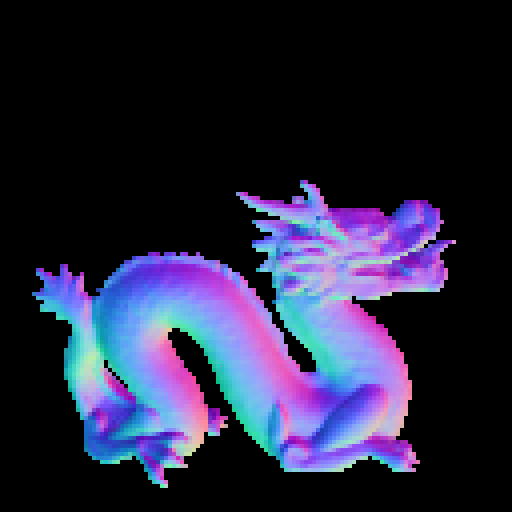
\includegraphics[width=\linewidth]{./Figures/visual_eval/fancy_eval_7_normal_GCNN-GCNN.png}
	\end{subfigure}
	
	\begin{subfigure}[b]{0.18\linewidth}
		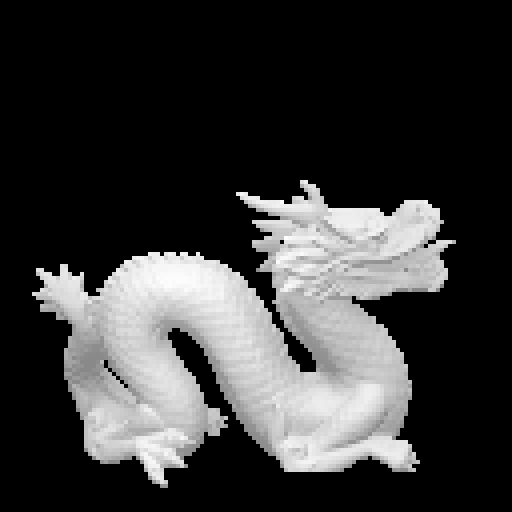
\includegraphics[width=\linewidth]{./Figures/visual_eval/fancy_eval_7_img.png}
		\caption{GT}
	\end{subfigure}
	\begin{subfigure}[b]{0.18\linewidth}
		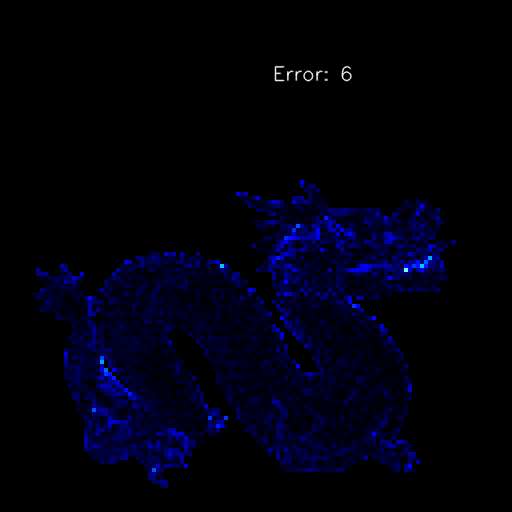
\includegraphics[width=\linewidth]{./Figures/visual_eval/fancy_eval_7_error_an2-8-1000.png}
		\caption{TripNet}
	\end{subfigure}
\begin{subfigure}[b]{0.18\linewidth}
	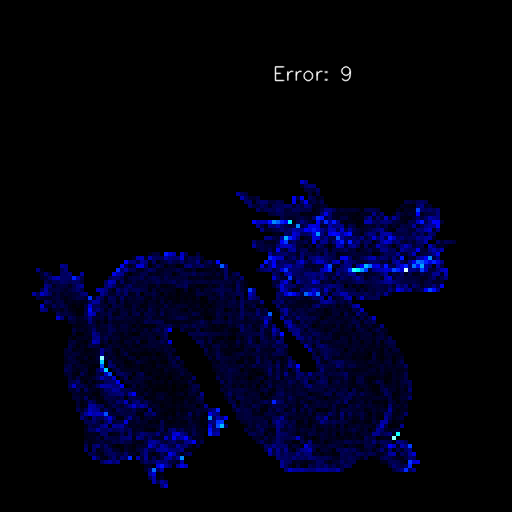
\includegraphics[width=\linewidth]{./Figures/visual_eval/fancy_eval_7_error_GCNN-GCNN.png}
	\caption{GCNN}
\end{subfigure}

	
	\begin{tikzpicture}
		\node[text width=0.1\textwidth] at (10,-1) {90};
		\node[inner sep=0pt] (input) at (8,-1)
		{
\includegraphics[width=.2\textwidth]{./Figures/colorscale_blue.png}};
		\node[text width=0.3\textwidth] at (7,-1) {Error: 0};
	\end{tikzpicture}
	
	\caption{TripNet qualitative evaluation. Surface Normal Inference on ``Dragon" object. The first row shows the estimated surface normal. The second row is the angle error map.}
	\label{fig:trip-eval}
\end{figure}

%% tripNet zoom in eval
\begin{figure}[H]
	\centering
	\begin{subfigure}[b]{0.18\linewidth}
		\includegraphics[width=\linewidth]{./Figures/visual_eval/eval_7_normal_GT.png}
	\end{subfigure}
	\begin{subfigure}[b]{0.18\linewidth}
		\includegraphics[width=\linewidth]{./Figures/visual_eval/eval_7_normal_an2-8-1000.png}
	\end{subfigure}
	\begin{subfigure}[b]{0.18\linewidth}
		\includegraphics[width=\linewidth]{./Figures/visual_eval/eval_7_normal_GCNN-GCNN.png}
	\end{subfigure}
	
	\begin{subfigure}[b]{0.18\linewidth}
		\includegraphics[width=\linewidth]{./Figures/visual_eval/eval_7_img.png}
		\caption{GT}
	\end{subfigure}
	\begin{subfigure}[b]{0.18\linewidth}
	\includegraphics[width=\linewidth]{./Figures/visual_eval/eval_7_error_an2-8-1000.png}
	\caption{Trip-Net}
	\end{subfigure}
	\begin{subfigure}[b]{0.18\linewidth}
		\includegraphics[width=\linewidth]{./Figures/visual_eval/eval_7_error_GCNN-GCNN.png}
		\caption{GCNN}
	\end{subfigure}

	
	\caption{Zoom in of the center region of Dragon object. The first row is surface normal, the second row is the corresponding errors.}
	\label{fig:tripnet-eval-synthetic-zoom-in}
\end{figure}


\begin{table}[th]
	
	\centering
	\begin{tabular}{l l l l l l l }
		\tabhead{Model} & \tabhead{Angle} & \tabhead{Time /ms} & \tabhead{bz} & \tabhead{lr-schedule} & \tabhead{lr-df} & \tabhead{l/i. Nr.}\\
		SVD  & 41.14  & 320.40 & - & - & - & 0 \\ 
		\hline
		GCNN  & 10.64 & 10.44 & 8 & 8,1000 & 0.5 & 0 \\
		\hline
		TripNet-CNN & 10.46 & 28.74 & 8 & 8,1000  & 0.5 & 1 \\
		\hline
		TripNet-F1B & 9.22 &44.59 & 8 & 8,1000  & 0.5 & 1 \\
		\hline
		TripNet & \textbf{9.17} & 43.79 & 8 & 8,1000  & 0.5 & 1 \\
	\end{tabular}
	\caption{A quantitative evaluation on proposed approaches. The angle error is the average angle error of all valid pixels in the test case. The time unit is in millisecond. bz is the batch size, lr-schedule is learning rate schedule. lr-df is learning rate decay factor, l/i. Nr is the number of light-image maps used for each scene}	
	\label{tab:model-error}
\end{table}




\subsection{Comparison}

\newpage
%% Final-Visual
\begin{figure}[H]
	\centering
	\begin{subfigure}[b]{0.24\linewidth}
		\includegraphics[width=\linewidth]{./Figures/visual_eval/fancy_eval_2_groundtruth.png}
	\end{subfigure}
	\begin{subfigure}[b]{0.24\linewidth}
		\includegraphics[width=\linewidth]{./Figures/visual_eval/fancy_eval_2_normal_an2-8-1000.png}
	\end{subfigure}
	\begin{subfigure}[b]{0.24\linewidth}
		\includegraphics[width=\linewidth]{./Figures/visual_eval/fancy_eval_2_normal_GCNN-GCNN.png}
	\end{subfigure}
	\begin{subfigure}[b]{0.24\linewidth}
	\includegraphics[width=\linewidth]{./Figures/visual_eval/fancy_eval_2_normal_SVD.png}
	\end{subfigure}

	\begin{subfigure}[b]{0.24\linewidth}
	\includegraphics[width=\linewidth]{./Figures/visual_eval/fancy_eval_2_img.png}
\end{subfigure}
\begin{subfigure}[b]{0.24\linewidth}
	\includegraphics[width=\linewidth]{./Figures/visual_eval/fancy_eval_2_error_an2-8-1000.png}
\end{subfigure}
\begin{subfigure}[b]{0.24\linewidth}
	\includegraphics[width=\linewidth]{./Figures/visual_eval/fancy_eval_2_error_GCNN-GCNN.png}
\end{subfigure}
\begin{subfigure}[b]{0.24\linewidth}
	\includegraphics[width=\linewidth]{./Figures/visual_eval/fancy_eval_2_error_SVD.png}
\end{subfigure}

	\begin{subfigure}[b]{0.24\linewidth}
	\includegraphics[width=\linewidth]{./Figures/visual_eval/fancy_eval_3_groundtruth.png}
\end{subfigure}
\begin{subfigure}[b]{0.24\linewidth}
	\includegraphics[width=\linewidth]{./Figures/visual_eval/fancy_eval_3_normal_an2-8-1000.png}
\end{subfigure}
\begin{subfigure}[b]{0.24\linewidth}
	\includegraphics[width=\linewidth]{./Figures/visual_eval/fancy_eval_3_normal_GCNN-GCNN.png}
\end{subfigure}
\begin{subfigure}[b]{0.24\linewidth}
	\includegraphics[width=\linewidth]{./Figures/visual_eval/fancy_eval_3_normal_SVD.png}
\end{subfigure}



\begin{subfigure}[b]{0.24\linewidth}
	\includegraphics[width=\linewidth]{./Figures/visual_eval/fancy_eval_3_img.png}
\end{subfigure}
\begin{subfigure}[b]{0.24\linewidth}
	\includegraphics[width=\linewidth]{./Figures/visual_eval/fancy_eval_3_error_an2-8-1000.png}
\end{subfigure}
\begin{subfigure}[b]{0.24\linewidth}
	\includegraphics[width=\linewidth]{./Figures/visual_eval/fancy_eval_3_error_GCNN-GCNN.png}
\end{subfigure}
\begin{subfigure}[b]{0.24\linewidth}
	\includegraphics[width=\linewidth]{./Figures/visual_eval/fancy_eval_3_error_SVD.png}
\end{subfigure}

	\begin{subfigure}[b]{0.24\linewidth}
	\includegraphics[width=\linewidth]{./Figures/visual_eval/fancy_eval_9_groundtruth.png}
\end{subfigure}
\begin{subfigure}[b]{0.24\linewidth}
	\includegraphics[width=\linewidth]{./Figures/visual_eval/fancy_eval_9_normal_an2-8-1000.png}
\end{subfigure}
\begin{subfigure}[b]{0.24\linewidth}
	\includegraphics[width=\linewidth]{./Figures/visual_eval/fancy_eval_9_normal_GCNN-GCNN.png}
\end{subfigure}
\begin{subfigure}[b]{0.24\linewidth}
	\includegraphics[width=\linewidth]{./Figures/visual_eval/fancy_eval_9_normal_SVD.png}
\end{subfigure}
	
	
\begin{subfigure}[b]{0.24\linewidth}
	\includegraphics[width=\linewidth]{./Figures/visual_eval/fancy_eval_9_img.png}
	\caption{GT}
\end{subfigure}
\begin{subfigure}[b]{0.24\linewidth}
	\includegraphics[width=\linewidth]{./Figures/visual_eval/fancy_eval_9_error_an2-8-1000.png}
	\caption{TripNet}
\end{subfigure}
\begin{subfigure}[b]{0.24\linewidth}
	\includegraphics[width=\linewidth]{./Figures/visual_eval/fancy_eval_9_error_GCNN-GCNN.png}
	\caption{GCNN}
\end{subfigure}
\begin{subfigure}[b]{0.24\linewidth}
	\includegraphics[width=\linewidth]{./Figures/visual_eval/fancy_eval_9_error_SVD.png}
	\caption{SVD}
\end{subfigure}
	
	
	\begin{tikzpicture}
		\node[text width=0.1\textwidth] at (10,-1) {90};
		\node[inner sep=0pt] (input) at (8,-1)
		{\includegraphics[width=.2\textwidth]{./Figures/colorscale_blue.png}};
		\node[text width=0.3\textwidth] at (7,-1) {Error: 0};
	\end{tikzpicture}
	
	\caption{Evaluation on objects Baoshanlu, Washington statue, Bus(from top to bottom).}
	\label{fig:final-eval}
\end{figure}


%% Final-Visual-Zoom-In
\begin{figure}[H]
	\centering
	\begin{subfigure}[b]{0.24\linewidth}
		\includegraphics[width=\linewidth]{./Figures/visual_eval/eval_2_normal_GT.png}
	\end{subfigure}
	\begin{subfigure}[b]{0.24\linewidth}
		\includegraphics[width=\linewidth]{./Figures/visual_eval/eval_2_normal_an2-8-1000.png}
	\end{subfigure}
	\begin{subfigure}[b]{0.24\linewidth}
		\includegraphics[width=\linewidth]{./Figures/visual_eval/eval_2_normal_GCNN-GCNN.png}
	\end{subfigure}
	\begin{subfigure}[b]{0.24\linewidth}
	\includegraphics[width=\linewidth]{./Figures/visual_eval/eval_2_normal_SVD.png}
	\end{subfigure}

	\begin{subfigure}[b]{0.24\linewidth}
	\includegraphics[width=\linewidth]{./Figures/visual_eval/eval_2_img.png}
\end{subfigure}
\begin{subfigure}[b]{0.24\linewidth}
	\includegraphics[width=\linewidth]{./Figures/visual_eval/eval_2_error_an2-8-1000.png}
\end{subfigure}
\begin{subfigure}[b]{0.24\linewidth}
	\includegraphics[width=\linewidth]{./Figures/visual_eval/eval_2_error_GCNN-GCNN.png}
\end{subfigure}
\begin{subfigure}[b]{0.24\linewidth}
	\includegraphics[width=\linewidth]{./Figures/visual_eval/eval_2_error_SVD.png}
\end{subfigure}




	\begin{subfigure}[b]{0.24\linewidth}
	\includegraphics[width=\linewidth]{./Figures/visual_eval/eval_3_normal_GT.png}
\end{subfigure}
\begin{subfigure}[b]{0.24\linewidth}
	\includegraphics[width=\linewidth]{./Figures/visual_eval/eval_3_normal_an2-8-1000.png}
\end{subfigure}
\begin{subfigure}[b]{0.24\linewidth}
	\includegraphics[width=\linewidth]{./Figures/visual_eval/eval_3_normal_GCNN-GCNN.png}
\end{subfigure}
\begin{subfigure}[b]{0.24\linewidth}
	\includegraphics[width=\linewidth]{./Figures/visual_eval/eval_3_normal_SVD.png}
\end{subfigure}

\begin{subfigure}[b]{0.24\linewidth}
	\includegraphics[width=\linewidth]{./Figures/visual_eval/eval_3_img.png}
\end{subfigure}
\begin{subfigure}[b]{0.24\linewidth}
	\includegraphics[width=\linewidth]{./Figures/visual_eval/eval_3_error_an2-8-1000.png}
\end{subfigure}
\begin{subfigure}[b]{0.24\linewidth}
	\includegraphics[width=\linewidth]{./Figures/visual_eval/eval_3_error_GCNN-GCNN.png}
\end{subfigure}
\begin{subfigure}[b]{0.24\linewidth}
	\includegraphics[width=\linewidth]{./Figures/visual_eval/eval_3_error_SVD.png}
\end{subfigure}



	\begin{subfigure}[b]{0.24\linewidth}
	\includegraphics[width=\linewidth]{./Figures/visual_eval/eval_9_normal_GT.png}
\end{subfigure}
\begin{subfigure}[b]{0.24\linewidth}
	\includegraphics[width=\linewidth]{./Figures/visual_eval/eval_9_normal_an2-8-1000.png}
\end{subfigure}
\begin{subfigure}[b]{0.24\linewidth}
	\includegraphics[width=\linewidth]{./Figures/visual_eval/eval_9_normal_GCNN-GCNN.png}
\end{subfigure}
\begin{subfigure}[b]{0.24\linewidth}
	\includegraphics[width=\linewidth]{./Figures/visual_eval/eval_9_normal_SVD.png}
\end{subfigure}

	
	\begin{subfigure}[b]{0.24\linewidth}
		\includegraphics[width=\linewidth]{./Figures/visual_eval/eval_9_img.png}
		\caption{GT}
	\end{subfigure}
	\begin{subfigure}[b]{0.24\linewidth}
		\includegraphics[width=\linewidth]{./Figures/visual_eval/eval_9_error_an2-8-1000.png}
		\caption{Trip-Net}
	\end{subfigure}
	\begin{subfigure}[b]{0.24\linewidth}
		\includegraphics[width=\linewidth]{./Figures/visual_eval/eval_9_error_GCNN-GCNN.png}
		\caption{GCNN}
	\end{subfigure}
		\begin{subfigure}[b]{0.24\linewidth}
		\includegraphics[width=\linewidth]{./Figures/visual_eval/eval_9_error_SVD.png}
		\caption{SVD}
	\end{subfigure}
	
	\caption{Zoom in of the center region of the objects in Figure \ref{fig:final-eval}}
	\label{fig:tripnet-eval-synthetic-zoom-in}
\end{figure}






From the Figure \ref{fig:normal-histo-diff} we can observe the normal difference between ground-truth and GCNN predicted normals in another dimension. It separates the interval $ \left[ -1,1 \right] $, which is exactly the range of normal vector, to 256 sections. Then it counts the number of points locates in each section for 3 axes.  The 3 axes are fitted quite well in most of interval but other than $ \left[ -0.25,0.25 \right] $ for x and y axes and  interval close to $ -1 $ for z axis. Therefore a further constraint can be considered to the loss function related to the normal difference shown in this figure.

It is faulty that almost no normal has -1 z-component in GCNN predicted normal map. The reason?



\subsection{Light Inpainting}
The light inpainting task in this section in order to evaluate the noise inpainting performance of GCNN model. It takes semi-dense light map as input to predict the fully dense light map, as shown in Figure \ref{fig:light-net-archi}. 
The network is trained on 3000 light maps in the "synthetic-50-5" dataset with initial learning rate 0.001, learning schedule 8,1000 with decay factor 0.5, the batch size is 8, the feature map channel is 128 in all of the gated convolution layers. All the models are tested on a laptop with a single NVIDIA GeForce 940MX, 2GB memory.

%% light eval model structure
\begin{figure}[th]
	\centering
	%% https://tex.stackexchange.com/questions/12020/what-is-the-easiest-way-to-draw-a-3d-cube-with-tikz
	\begin{tikzpicture}
		%% -------------------------------------- parameters ------------------------------------------------
		\pgfmathsetmacro{\vdist}{0.4}
		
		\pgfmathsetmacro{\boxsizea}{2}	%% width 512
		\pgfmathsetmacro{\boxwidtha}{2}	%% width 3
		
		%% https://www.tug.org/pracjourn/2007-4/walden/color.pdf
		\definecolor{netcolor}{rgb}{0.5,0.7,0.7}
		
		%% 	d_in							3x512x512
		%%	dconv1: 	d_in-->x1 			32x512x512
		\pgfmathsetmacro{\disttimes}{1}	%% width 32
		\pgfmathsetmacro{\yshift}{1}	%% width 32
		\pgfmathsetmacro{\boxsize}{\boxsizea}	%% size 512
		\pgfmathsetmacro{\boxwidth}{\boxwidtha}	%% width 32
		\pgfmathsetmacro{\yschift}{-1}
		
		
		\node[inner sep=0pt] (input) at (\vdist*\disttimes-6,\yschift-0.8)
		{\includegraphics[width=.2\textwidth]{./Figures/gcnn-synthetic/intrinsic_image_light_input.png}};
		\node[text width=3.5cm] at (\vdist*\disttimes-6,\yschift-2.4) {Semi-dense Light Map};
		
		\node[inner sep=0pt] (output) at (\vdist*\disttimes+3,\yschift-0.8)
		{\includegraphics[width=.2\textwidth]{./Figures/gcnn-synthetic/intrinsic_image_light.png}};
		\node[text width=3.5cm] at (\vdist*\disttimes+3,\yschift-2.4) {fully-dense Light Map};
		
		\draw [-stealth] (\vdist*\disttimes-4.5,\yschift-1) -- (\vdist*\disttimes-3.5,\yschift-1);
		\draw [-stealth] (\vdist*\disttimes,\yschift-1) -- (\vdist*\disttimes+1,\yschift-1);
		
		
		\pgfmathsetmacro{\disttimes}{-2}	%% width 32		
		\pgfmathsetmacro{\yschift}{-1}
		\draw[black, fill=netcolor] (\vdist*\disttimes,\yschift,0) -- ++(-\boxwidth,0,0) -- ++(0,-\boxsize,0) -- ++(\boxwidth,0,0) -- cycle;
		\draw[black, fill=netcolor] (\vdist*\disttimes,\yschift,0) -- ++(0,0,-\boxsize) -- ++(0,-\boxsize,0) -- ++(0,0,\boxsize) -- cycle;
		\draw[black, fill=netcolor] (\vdist*\disttimes,\yschift,0) -- ++(-\boxwidth,0,0) -- ++(0,0,-\boxsize) -- ++(\boxwidth,0,0) -- cycle;
		
		\node[text width=3.5cm] at (\vdist*\disttimes+0.3,\yschift-1) {GCNN};
	\end{tikzpicture}
	\caption{Light map inpainting based on GCNN architecture.}
	\label{fig:light-net-archi}
\end{figure}

The result is shown in Table \ref{tab:light-inpainting}. Besides the GCNN model, we use two extra model as the comparisons. The first one is GCNN-NOC, where NOC means "no skip connection", the second one is CNN, which has the same architecture as the GCNN but only use standard convolution layers in the network.
The GCNN architecture achieves the average angle error lower than 1 degree. As a comparison, U-CNN model has 4 degrees error, which shows the relative weakness of noise filter competence. Besides, the skip connection also booster the performance, since the no skip connection version still has error greater than 1 degree. The both two models for the inpainting task reveals the superiority of GCNN architecture. Figure \ref{fig:light-scatter} and \ref{fig:light-eval} gives a quantitative and qualitative evaluation.

%% light eval table
\begin{table}[H]
	
	\centering
	\begin{tabular}{l l l l l l }
		\tabhead{Model} & \tabhead{Angle} & \tabhead{Time /ms} & \tabhead{bz} & \tabhead{lr-schedule} & \tabhead{lr-df}\\
		U-GCNN  & 0.59  & 14.45 & 8 & 8,1000 & 0.5\\ 
		\hline
		U-GCNN-NOC & 1.31 & 16.14 & 8 & 8,1000 & 0.5\\
		\hline
		U-CNN & 4.10 & 10.52 & 8 & 8,1000 & 0.5\\
	\end{tabular}
	\caption{The performance of the GCNN model for light map inpainting. The angle error is the average angle error of all valid pixels in the test case. bz stands for batch size, lr-schedule stands for learning rate schedule, lr-df stands for learning rate decay factor.}	
	\label{tab:light-inpainting}
\end{table}


%% light eval visualization
\begin{figure}[H]
	\centering
	\begin{subfigure}[b]{0.24\linewidth}
		\includegraphics[width=\linewidth]{./Figures/visual_eval/fancy_eval_7_img.png}
		\caption{gray-scale image}
	\end{subfigure}
	\begin{subfigure}[b]{0.24\linewidth}
		\includegraphics[width=\linewidth]{./Figures/visual_eval/fancy_eval_7_light_input.png}
		\caption{Light Direction}
	\end{subfigure}
	\begin{subfigure}[b]{0.24\linewidth}
		\includegraphics[width=\linewidth]{./Figures/visual_eval/fancy_eval_7_light_gt.png}
		\caption{ground-truth}
	\end{subfigure}
	
	\begin{subfigure}[b]{0.24\linewidth}
		\includegraphics[width=\linewidth]{./Figures/visual_eval/fancy_eval_7_light_light-gcnn.png}
		\caption{GCNN}
	\end{subfigure}
	\begin{subfigure}[b]{0.24\linewidth}
		\includegraphics[width=\linewidth]{./Figures/visual_eval/fancy_eval_7_light_light-cnn.png}
		\caption{U-CNN}
	\end{subfigure}
	\begin{subfigure}[b]{0.24\linewidth}
		\includegraphics[width=\linewidth]{./Figures/visual_eval/fancy_eval_7_light_light-noc.png}
		\caption{U-GCNN-NOC}
	\end{subfigure}
	
	\begin{subfigure}[b]{0.24\linewidth}
		\includegraphics[width=\linewidth]{./Figures/visual_eval/fancy_eval_7_light_error_light-gcnn.png}
		\caption{U-GCNN Error}
	\end{subfigure}
	\begin{subfigure}[b]{0.24\linewidth}
		\includegraphics[width=\linewidth]{./Figures/visual_eval/fancy_eval_7_light_error_light-cnn.png}
		\caption{U-CNN Error}
	\end{subfigure}
	\begin{subfigure}[b]{0.24\linewidth}
		\includegraphics[width=\linewidth]{./Figures/visual_eval/fancy_eval_7_light_error_light-noc.png}
		\caption{U-NOC Error}
	\end{subfigure}
	
	\begin{tikzpicture}
		\node[text width=0.1\textwidth] at (10,-1) {90};
		\node[inner sep=0pt] (input) at (8,-1)
		{\includegraphics[width=.2\textwidth]{./Figures/colorscale_hot-vertical.jpg}};
		\node[text width=0.3\textwidth] at (7,-1) {Error: 0};
	\end{tikzpicture}
	
	\caption{GCNN Normal Inference for light map inpainting based on dragon object. The degree error map is shown in last row. The average error is shown in the upper right corner in the error map.}
	\label{fig:light-eval}
\end{figure}

%% light eval scatter
\begin{figure}[H]
	\centering
	\includegraphics[width=0.9\linewidth]{./Figures/gcnn-light/scatter-light.png}
	\caption{GCNN for light map inpainting on 100 scenes. The evaluated models are corresponding to the table \ref{tab:light-inpainting}, the line in the figure is the corresponding regression line of each model.}
	\label{fig:light-scatter}
\end{figure}


The evaluation visualization on real dataset is shown in Figure \ref{fig:gcnn-eval-real}
%% fig:gcnn-eval-real
\begin{figure}[th]
	\centering
	\begin{subfigure}[b]{0.24\linewidth}
		\includegraphics[width=\linewidth]{./Figures/gcnn-real/fancy_eval_1_point_cloud_noise.png}
		\caption{point cloud}
	\end{subfigure}
	\begin{subfigure}[b]{0.24\linewidth}
		\includegraphics[width=\linewidth]{./Figures/gcnn-real/fancy_eval_1_groundtruth.png}
		\caption{ground-truth}
	\end{subfigure}
	\begin{subfigure}[b]{0.24\linewidth}
		\includegraphics[width=\linewidth]{./Figures/gcnn-real/fancy_eval_1_normal_GCNN.png}
		\caption{GCNN}
	\end{subfigure}
	\begin{subfigure}[b]{0.24\linewidth}
		\includegraphics[width=\linewidth]{./Figures/gcnn-real/fancy_eval_1_error_GCNN.png}
		\caption{Angle Error}
	\end{subfigure}
	\caption{Evaluation on Real Dataset}
	\label{fig:gcnn-eval-real}
\end{figure}


We evaluate the U-GCNN model on 100 test images as a quantitative evaluation. The result is shown in Figure \ref{fig:scatter-gcnn}. The GCNN based method has average angle error around 10 degrees, whereas the no skip connection version has error above 12 degrees and the CNN version has error above 15 degrees.

%% scatter_gcnn
\begin{figure}[h!]
	\centering
	\includegraphics[width=.8\textwidth]{./Figures/gcnn-synthetic/gcnn-scatter.png}
	\caption{Evaluation of average angular loss on the whole test dataset with 100 scenes. The x-axis indicates the point number, the y-axis indicates the angles. The lines show in the picture are the regression line of each model.}
	\label{fig:scatter-gcnn}
\end{figure}




\end{document}
